
\section{4+8f, $\beta = 4.0$, $24^3$, $m_\ell = 0.015, m_h = 0.080$}

$N_{meas} = 2000$, Autocorrelation of 2 measurements (40 MDTU), $N = 1000$. $M_\pi = 0$, $F_\pi = 0$, $M_\rho = 0$, $M_{axial} = 0$, $M_{a_0} = 0$, $M_{nu+} = 0$. 



\begin{multicols}{2}
	\begin{figure}[H]
\centering
        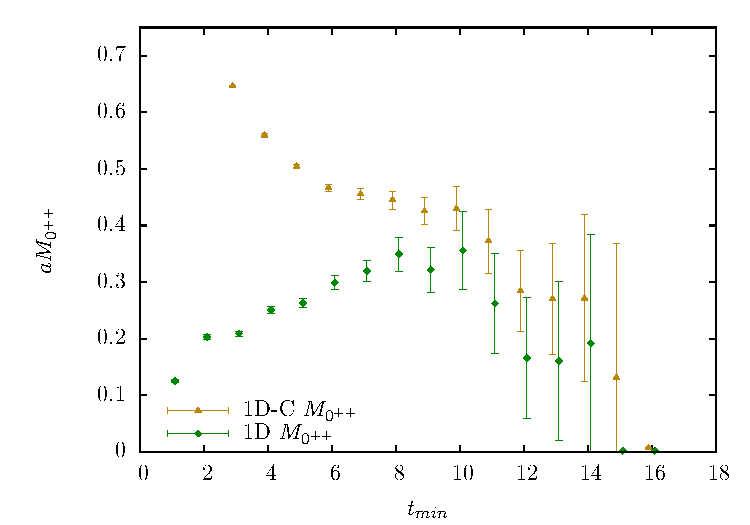
\includegraphics[width=2.5in]{./f4plus8l24t48b40m015m080/plots/m0pp_zcen_cmp.pdf}\\
	\caption{Masses from non-linear fits from $t_{min}$ to the center of the correlator $N_t/2$.}
\end{figure}
\columnbreak
\begin{figure}[H]
\centering
    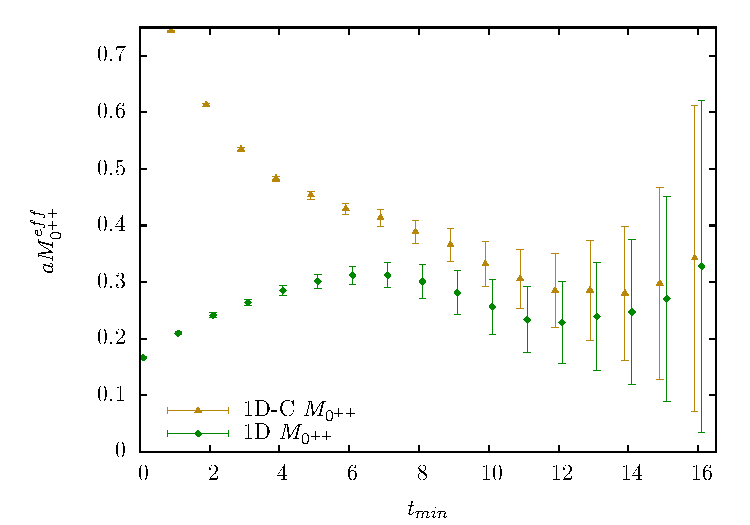
\includegraphics[width=2.5in]{./f4plus8l24t48b40m015m080/plots/m0pp_zcen_eff.pdf}\\
	\caption{Kuti-style effective mass plots. }
\end{figure}
\end{multicols}

\begin{multicols}{2}
	\begin{figure}[H]
\centering
        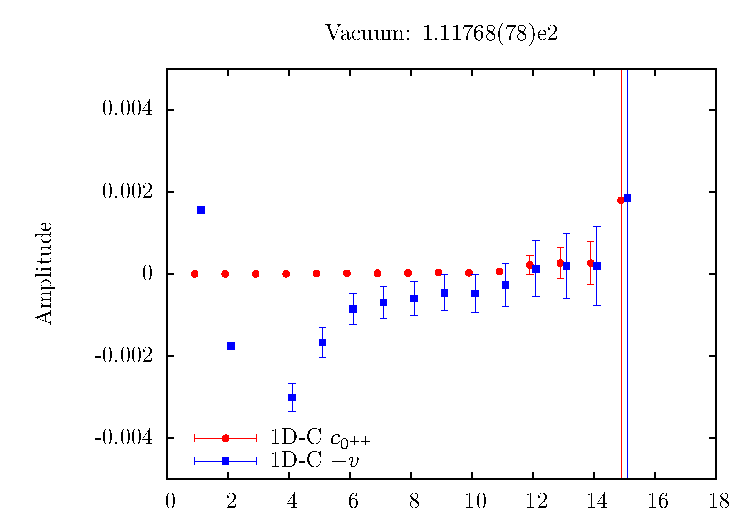
\includegraphics[width=2.5in]{./f4plus8l24t48b40m015m080/plots/m0pp_zcen_amp.pdf}\\
	\caption{Amplitude and vacuum comparison (1D-C) from non-linear fits from $t_{min}$ to the center of the correlator $N_t/2$.}
\end{figure}
\columnbreak
\begin{figure}[H]
\centering
    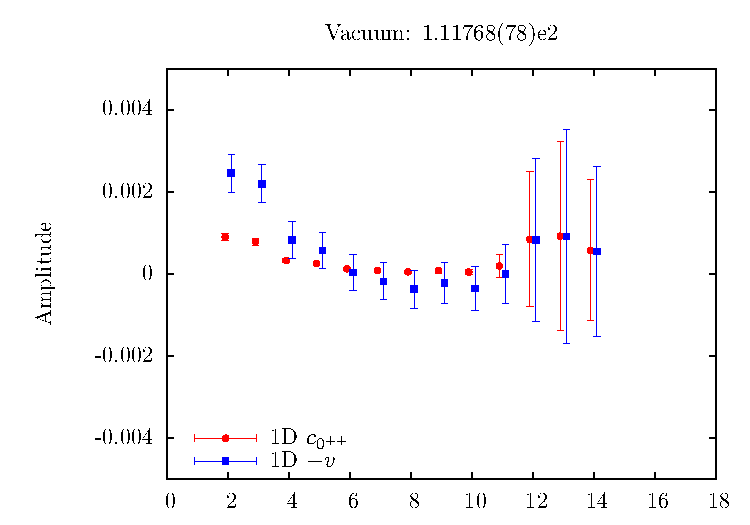
\includegraphics[width=2.5in]{./f4plus8l24t48b40m015m080/plots/m0pp_zcen_amp_dc.pdf}\\
	\caption{Amplitude and vacuum comparison (1D) from non-linear fits from $t_{min}$ to the center of the correlator $N_t/2$.}
\end{figure}
\end{multicols}

\begin{multicols}{2}
	\begin{figure}[H]
\centering
        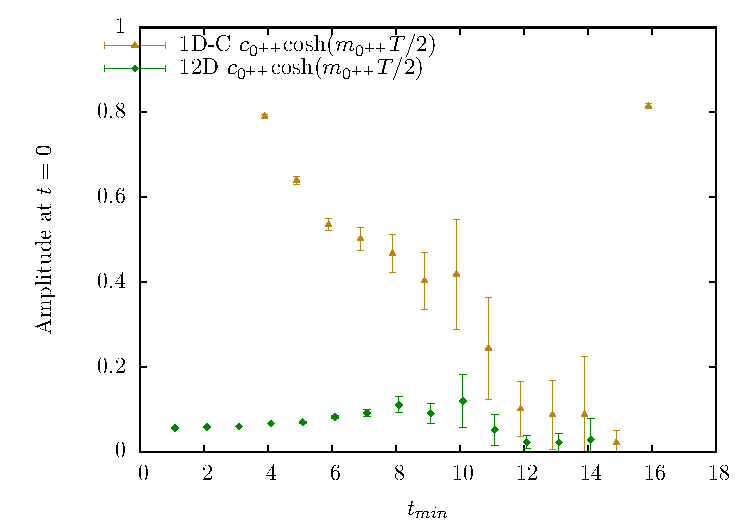
\includegraphics[width=2.5in]{./f4plus8l24t48b40m015m080/plots/m0pp_zcen_amp_orig.pdf}\\
	\caption{Amplitude (propagated back to $t=0$) from non-linear fits from $t_{min}$ to the center of the correlator $N_t/2$.}
\end{figure}
\columnbreak
\begin{figure}[H]
\centering
        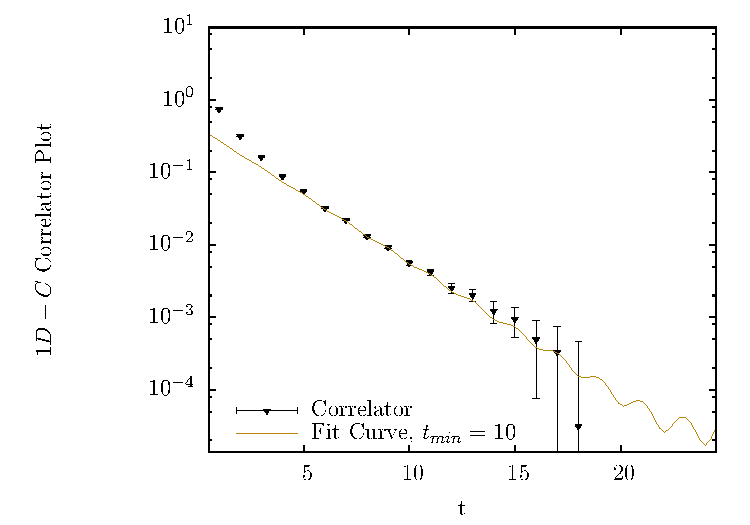
\includegraphics[width=2.5in]{./f4plus8l24t48b40m015m080/plots/m0pp_zcen_fitlines.pdf}\\
        \caption{A sample fit of the data to a fit form. We look at 1D-C using results from $t_{min} = 10$.}
\end{figure}

\end{multicols}

